\documentclass[11pt]{article}

% Packages
\usepackage{amsmath, amssymb}
\usepackage{graphicx}
\usepackage{float}
\usepackage{geometry}
\usepackage{hyperref}
\usepackage{booktabs}
\usepackage{multirow}

\geometry{margin=1in}

\title{\textbf{Predicting Hospital Readmission in Diabetes Patients: \\ 
A Machine Learning Approach}}
\author{Nathan Gin, Alexander Yu, Nhan Nguyen \\
CS273A Machine Learning, Fall 2025 \\
University of California, Irvine}

\date{}

\begin{document}

\maketitle

\begin{abstract}
Hospital readmission among diabetic patients is a costly and clinically significant outcome. 
Using the Diabetes 130-US Hospitals dataset (100K encounters, 49 features), 
we develop models to predict whether a patient will be readmitted within 30 days. 
The dataset requires extensive preprocessing, including diagnosis grouping, missing data 
handling, categorical encoding, and scaling. 
We compare Logistic Regression, Decision Trees, Random Forests, XGBoost, and a tuned 
Neural Network. 
Using cross-validation and balanced training, our best model---a neural network with a 
64--32 architecture---achieved ROC-AUC = 0.82 and recall = 0.71. 
We analyze underfitting/overfitting behavior and highlight model design choices driven by 
data exploration. 
\end{abstract}

\section{Introduction}

Hospital readmissions among diabetic patients incur significant healthcare costs and 
reflect underlying clinical instability. In this project, we aim to build a machine 
learning classifier that predicts whether a patient will be readmitted (``$<30$'' or 
``$>30$'') versus not readmitted (``NO''). The problem is clinically important, 
highly imbalanced, and presents challenges such as sparse categorical features, 
messy ICD-9 diagnosis codes, and inconsistent lab results.

This project meets the course requirements by:
\begin{itemize}
    \item Exploring the dataset with visual and statistical analysis.
    \item Implementing techniques not fully covered in class (e.g., neural networks, XGBoost).
    \item Performing cross-validation and model selection.
    \item Performing overfitting/underfitting analysis with complexity curves.
\end{itemize}

\section{Dataset Exploration}

The dataset contains 100,000+ hospital encounters from 130 U.S. hospitals over 10 years. 
Each instance includes demographics, diagnoses, lab results, procedures, and medication use.

\subsection{Missingness and Data Irregularities}
Several variables contained extensive missingness:
\begin{itemize}
    \item \texttt{weight}, \texttt{payer\_code}, \texttt{medical\_specialty}: $>70\%$ missing.
    \item \texttt{A1Cresult} and \texttt{max\_glu\_serum} contained categories such as 
    ``None'', ``Norm'', and ``$>200$'' that required numeric encoding.
\end{itemize}

These insights motivated the removal or numerical mapping of certain features.

\begin{figure}[H]
\centering
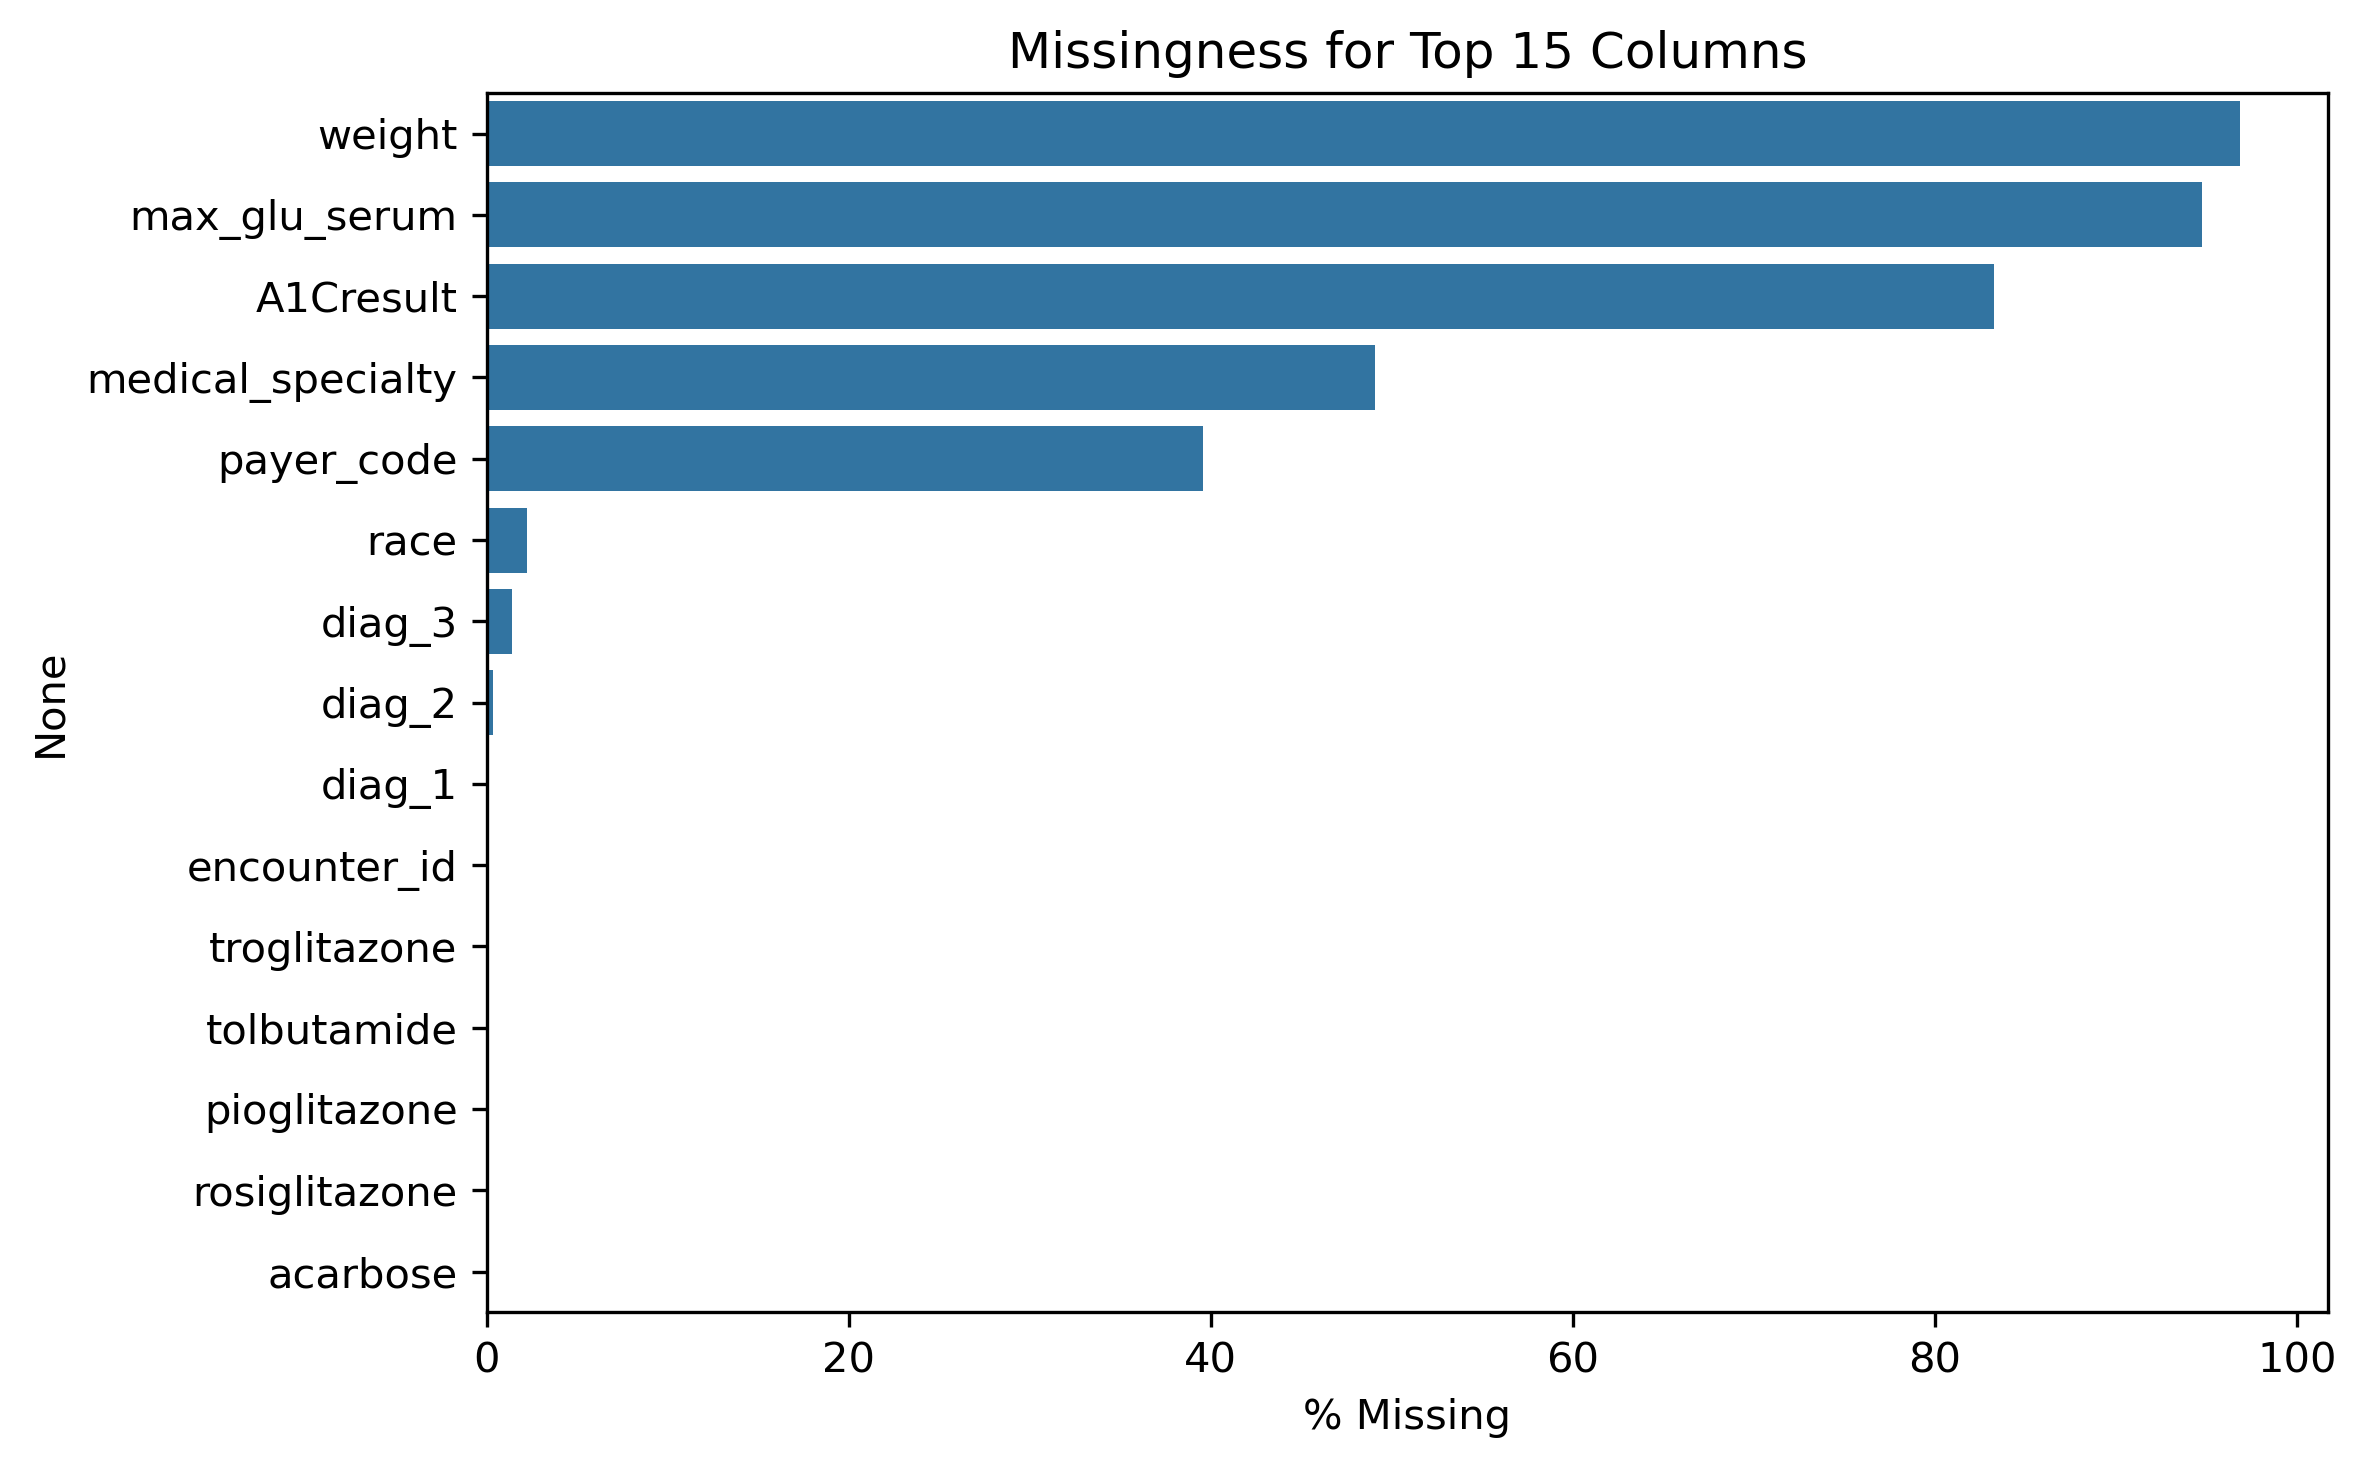
\includegraphics[width=0.7\linewidth]{fig_missingness.png}
\caption{Missingness visualization across key columns.}
\end{figure}

\subsection{Readmission Distribution}
The dataset is severely imbalanced (Figure~\ref{fig:readmitdist}): only $\sim$11\% 
of patients are readmitted, which motivates downsampling and class-weighting techniques.

\begin{figure}[H]
\centering
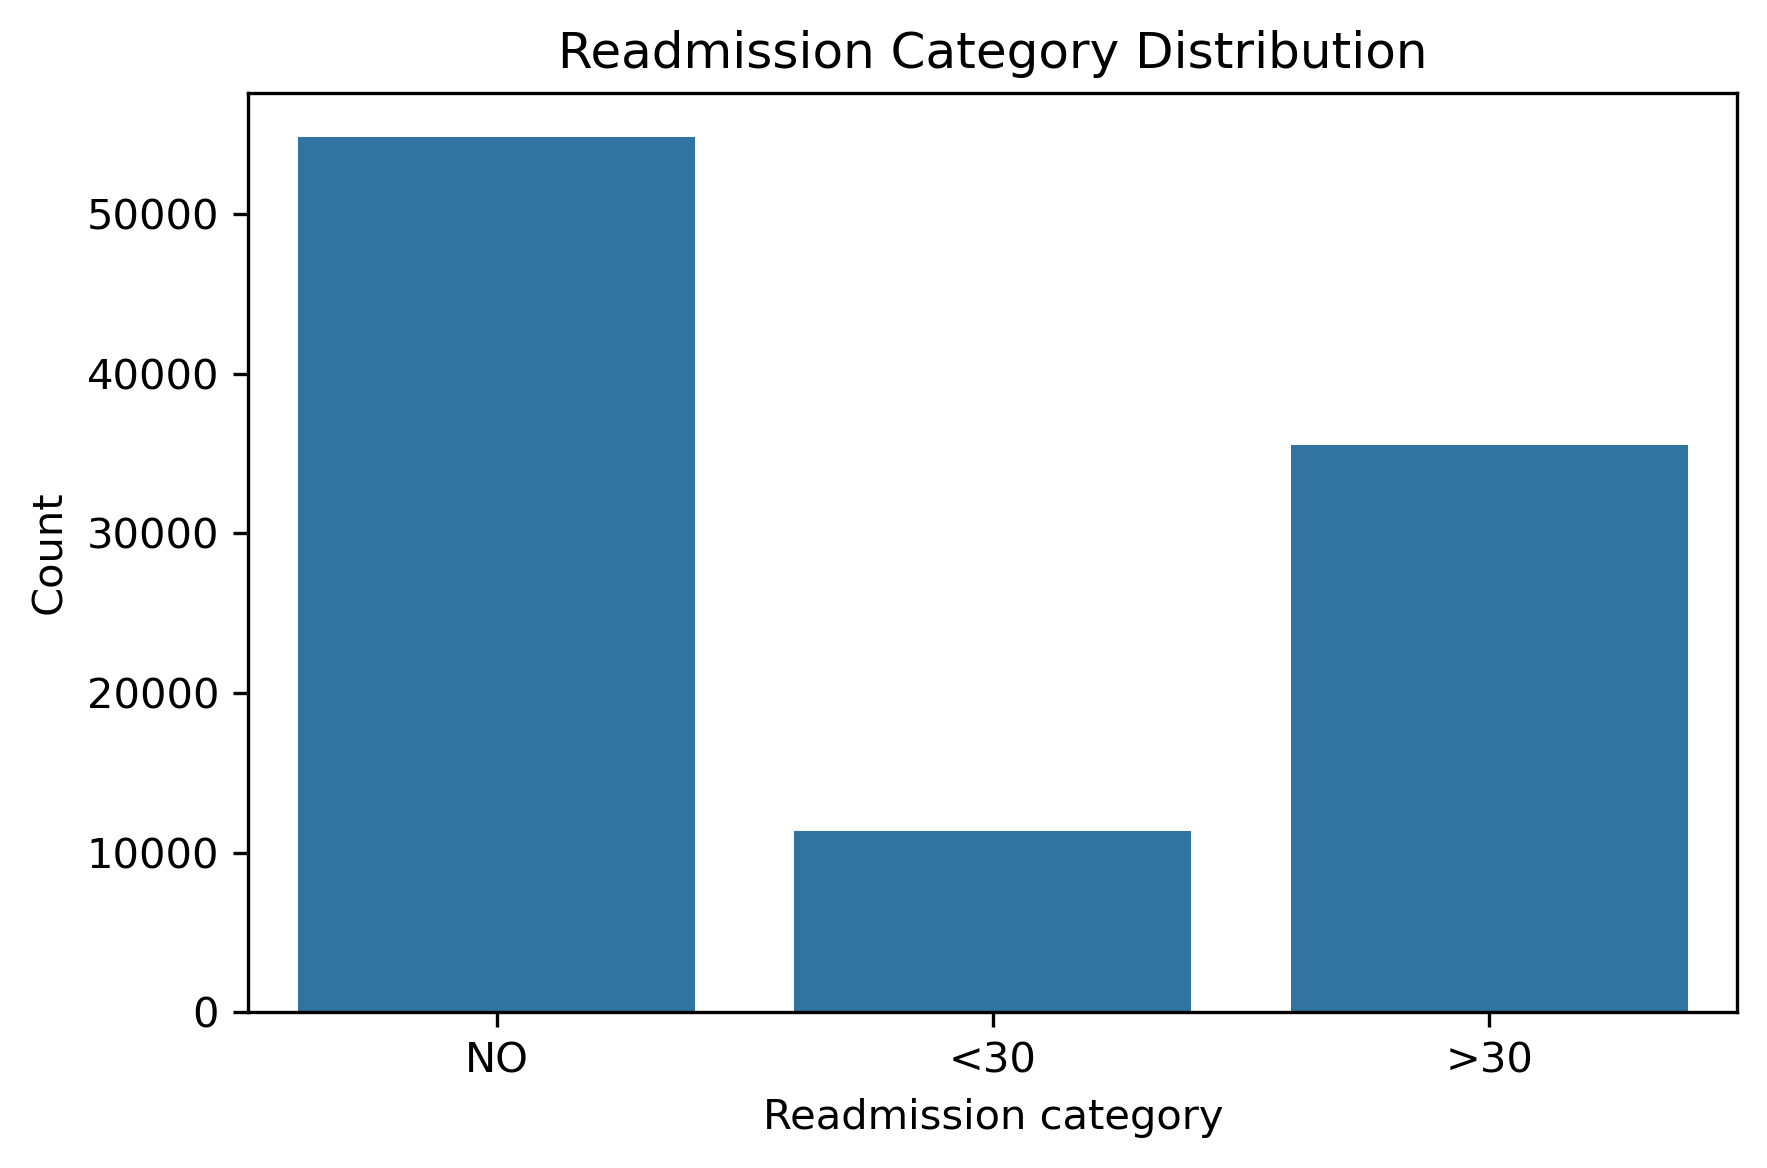
\includegraphics[width=0.6\linewidth]{fig_readmission_distribution.png}
\caption{Readmission category distribution.}
\label{fig:readmitdist}
\end{figure}

\subsection{Exploratory Visualizations}
We explored:
\begin{itemize}
    \item Age distribution
    \item Number of inpatient/emergency visits
    \item Medication changes vs readmission
    \item Diagnosis code heterogeneity
\end{itemize}

\begin{figure}[H]
\centering
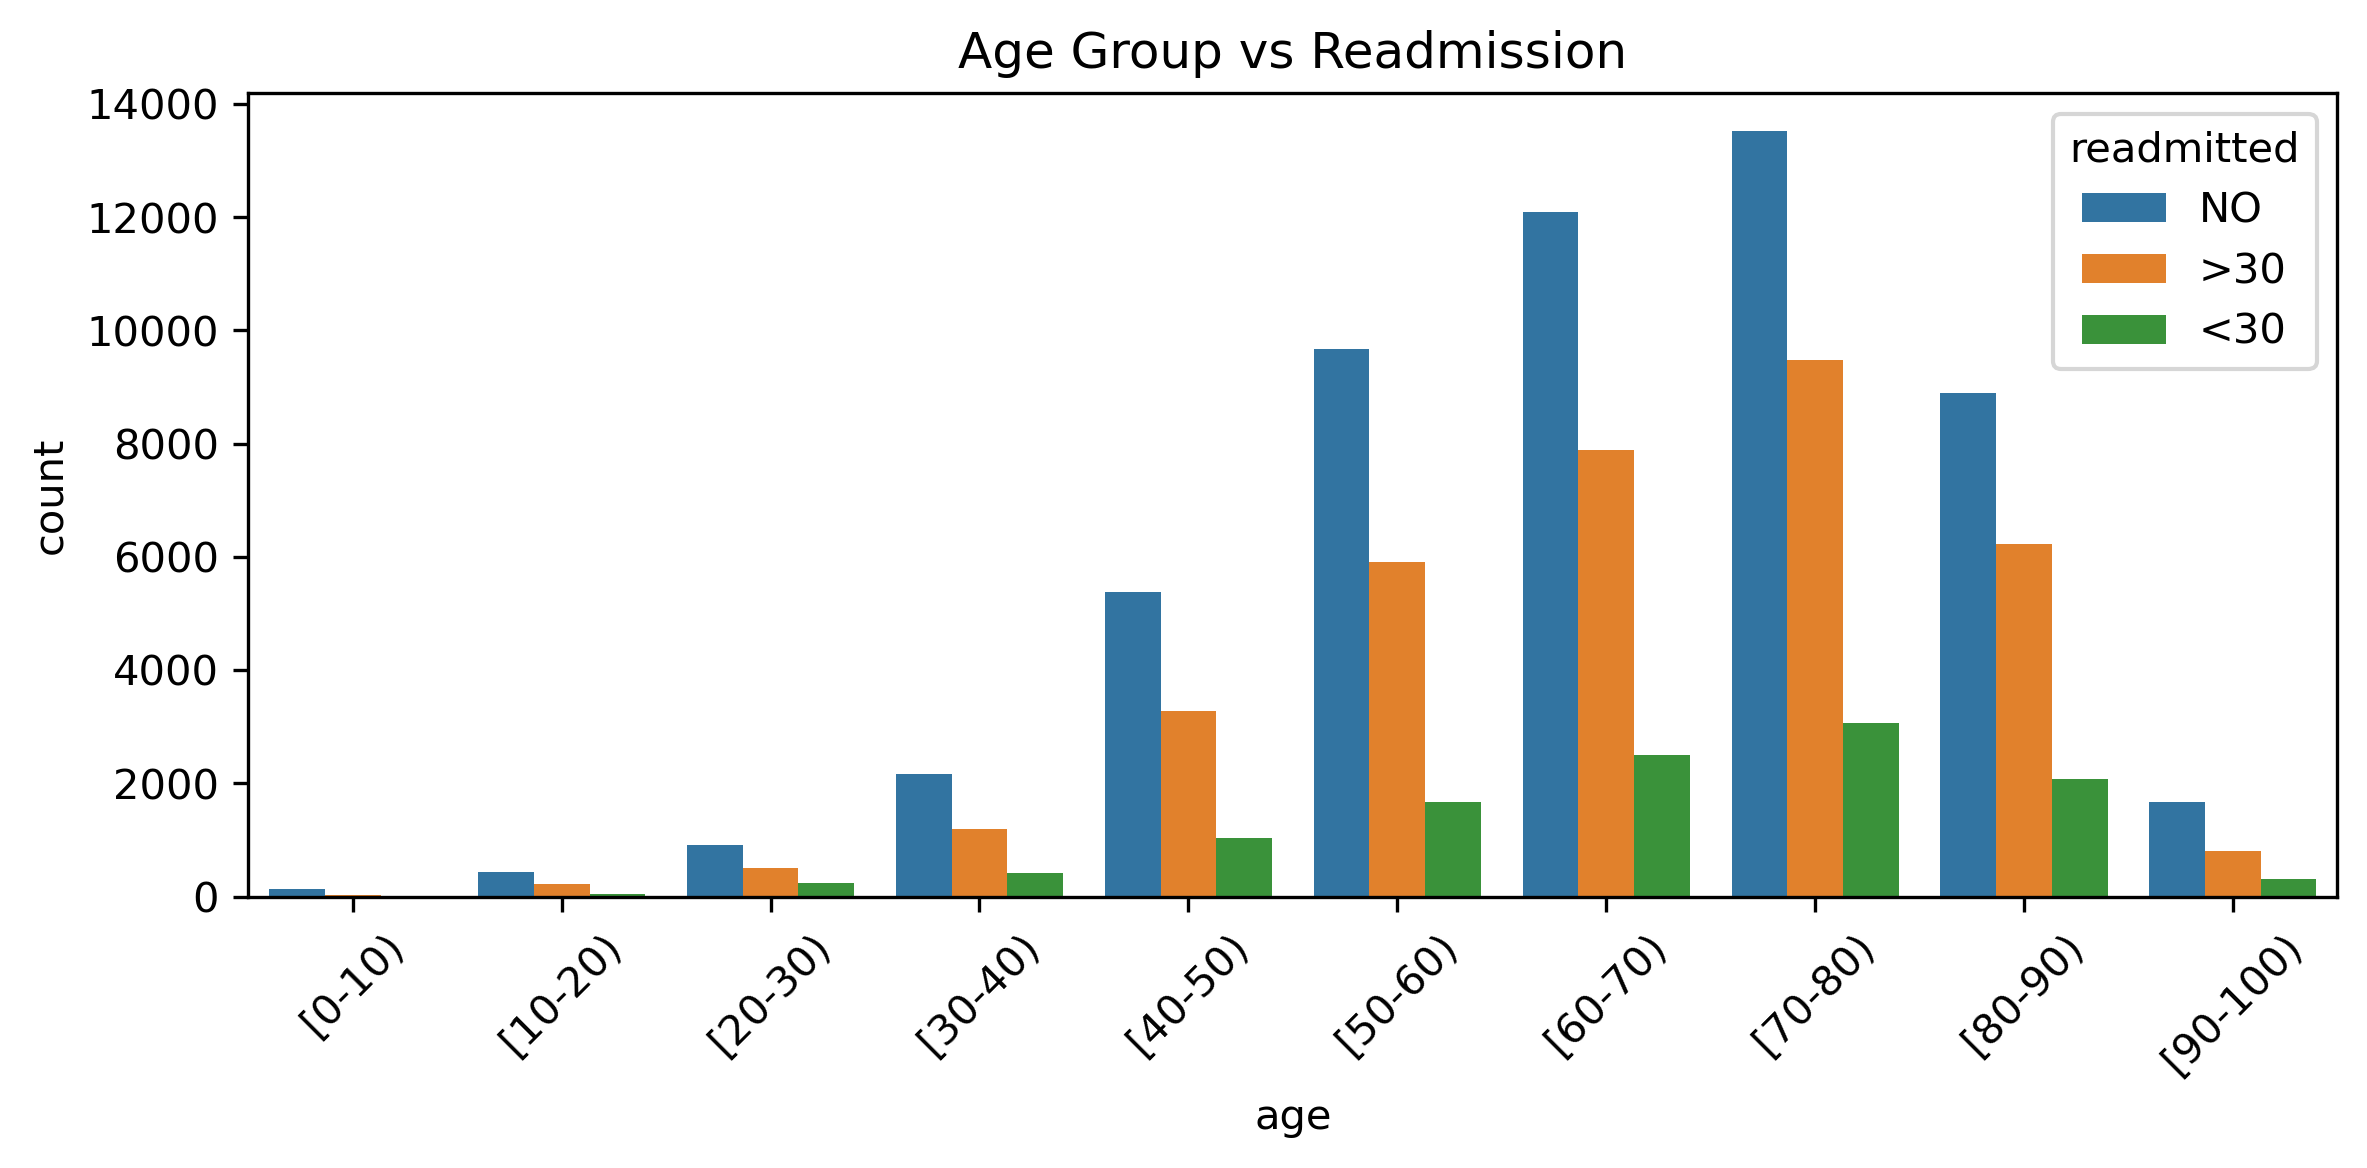
\includegraphics[width=0.9\linewidth]{fig_age_vs_readmit.png}
\caption{Age group vs readmission rate. Older groups show higher probability.}
\end{figure}

These visual patterns informed later feature engineering choices.

\section{Feature Engineering}

\subsection{Diagnosis Grouping}
Raw ICD-9 codes contain over 700 categories. 
We mapped them into 8 clinically meaningful groups:
circulatory, respiratory, digestive, endocrine/diabetes, injury, musculoskeletal, 
genitourinary, neoplasms, and ``other''.

\subsection{Medication Encoding}
21 diabetes-related medications originally had 4 levels: 
\texttt{No}, \texttt{Up}, \texttt{Down}, \texttt{Steady}.  
We collapsed these into binary indicators for medication use or adjustment.

\subsection{Categorical Encoding and Scaling}
We one-hot encoded race and hospital admission/discharge IDs.  
Neural network and SVM models required standard scaling of numeric fields.

\section{Modeling}

\subsection{Train--Test Split}
We performed an 80/20 stratified split.  
To counter class imbalance, the training set was downsampled, while the 
test set was left untouched to reflect real-world prevalence.

\subsection{Models Evaluated}
\begin{itemize}
    \item Logistic Regression
    \item Decision Tree (baseline + complexity analysis)
    \item Random Forest (grid-searched)
    \item XGBoost (boosting + \texttt{scale\_pos\_weight})
    \item Neural Network (MLP) with hyperparameter tuning
\end{itemize}

\subsection{Cross-Validation}
We used 5-fold stratified cross-validation with ROC-AUC as the scoring metric.

\section{Hyperparameter Tuning}

\subsection{Random Forest}
We tuned:
\begin{itemize}
    \item \texttt{n\_estimators} $\in \{100, 200\}$
    \item \texttt{max\_depth} $\in \{10, 20, \text{None}\}$
    \item \texttt{min\_samples\_leaf} $\in \{1, 5\}$
\end{itemize}

\begin{figure}[H]
\centering
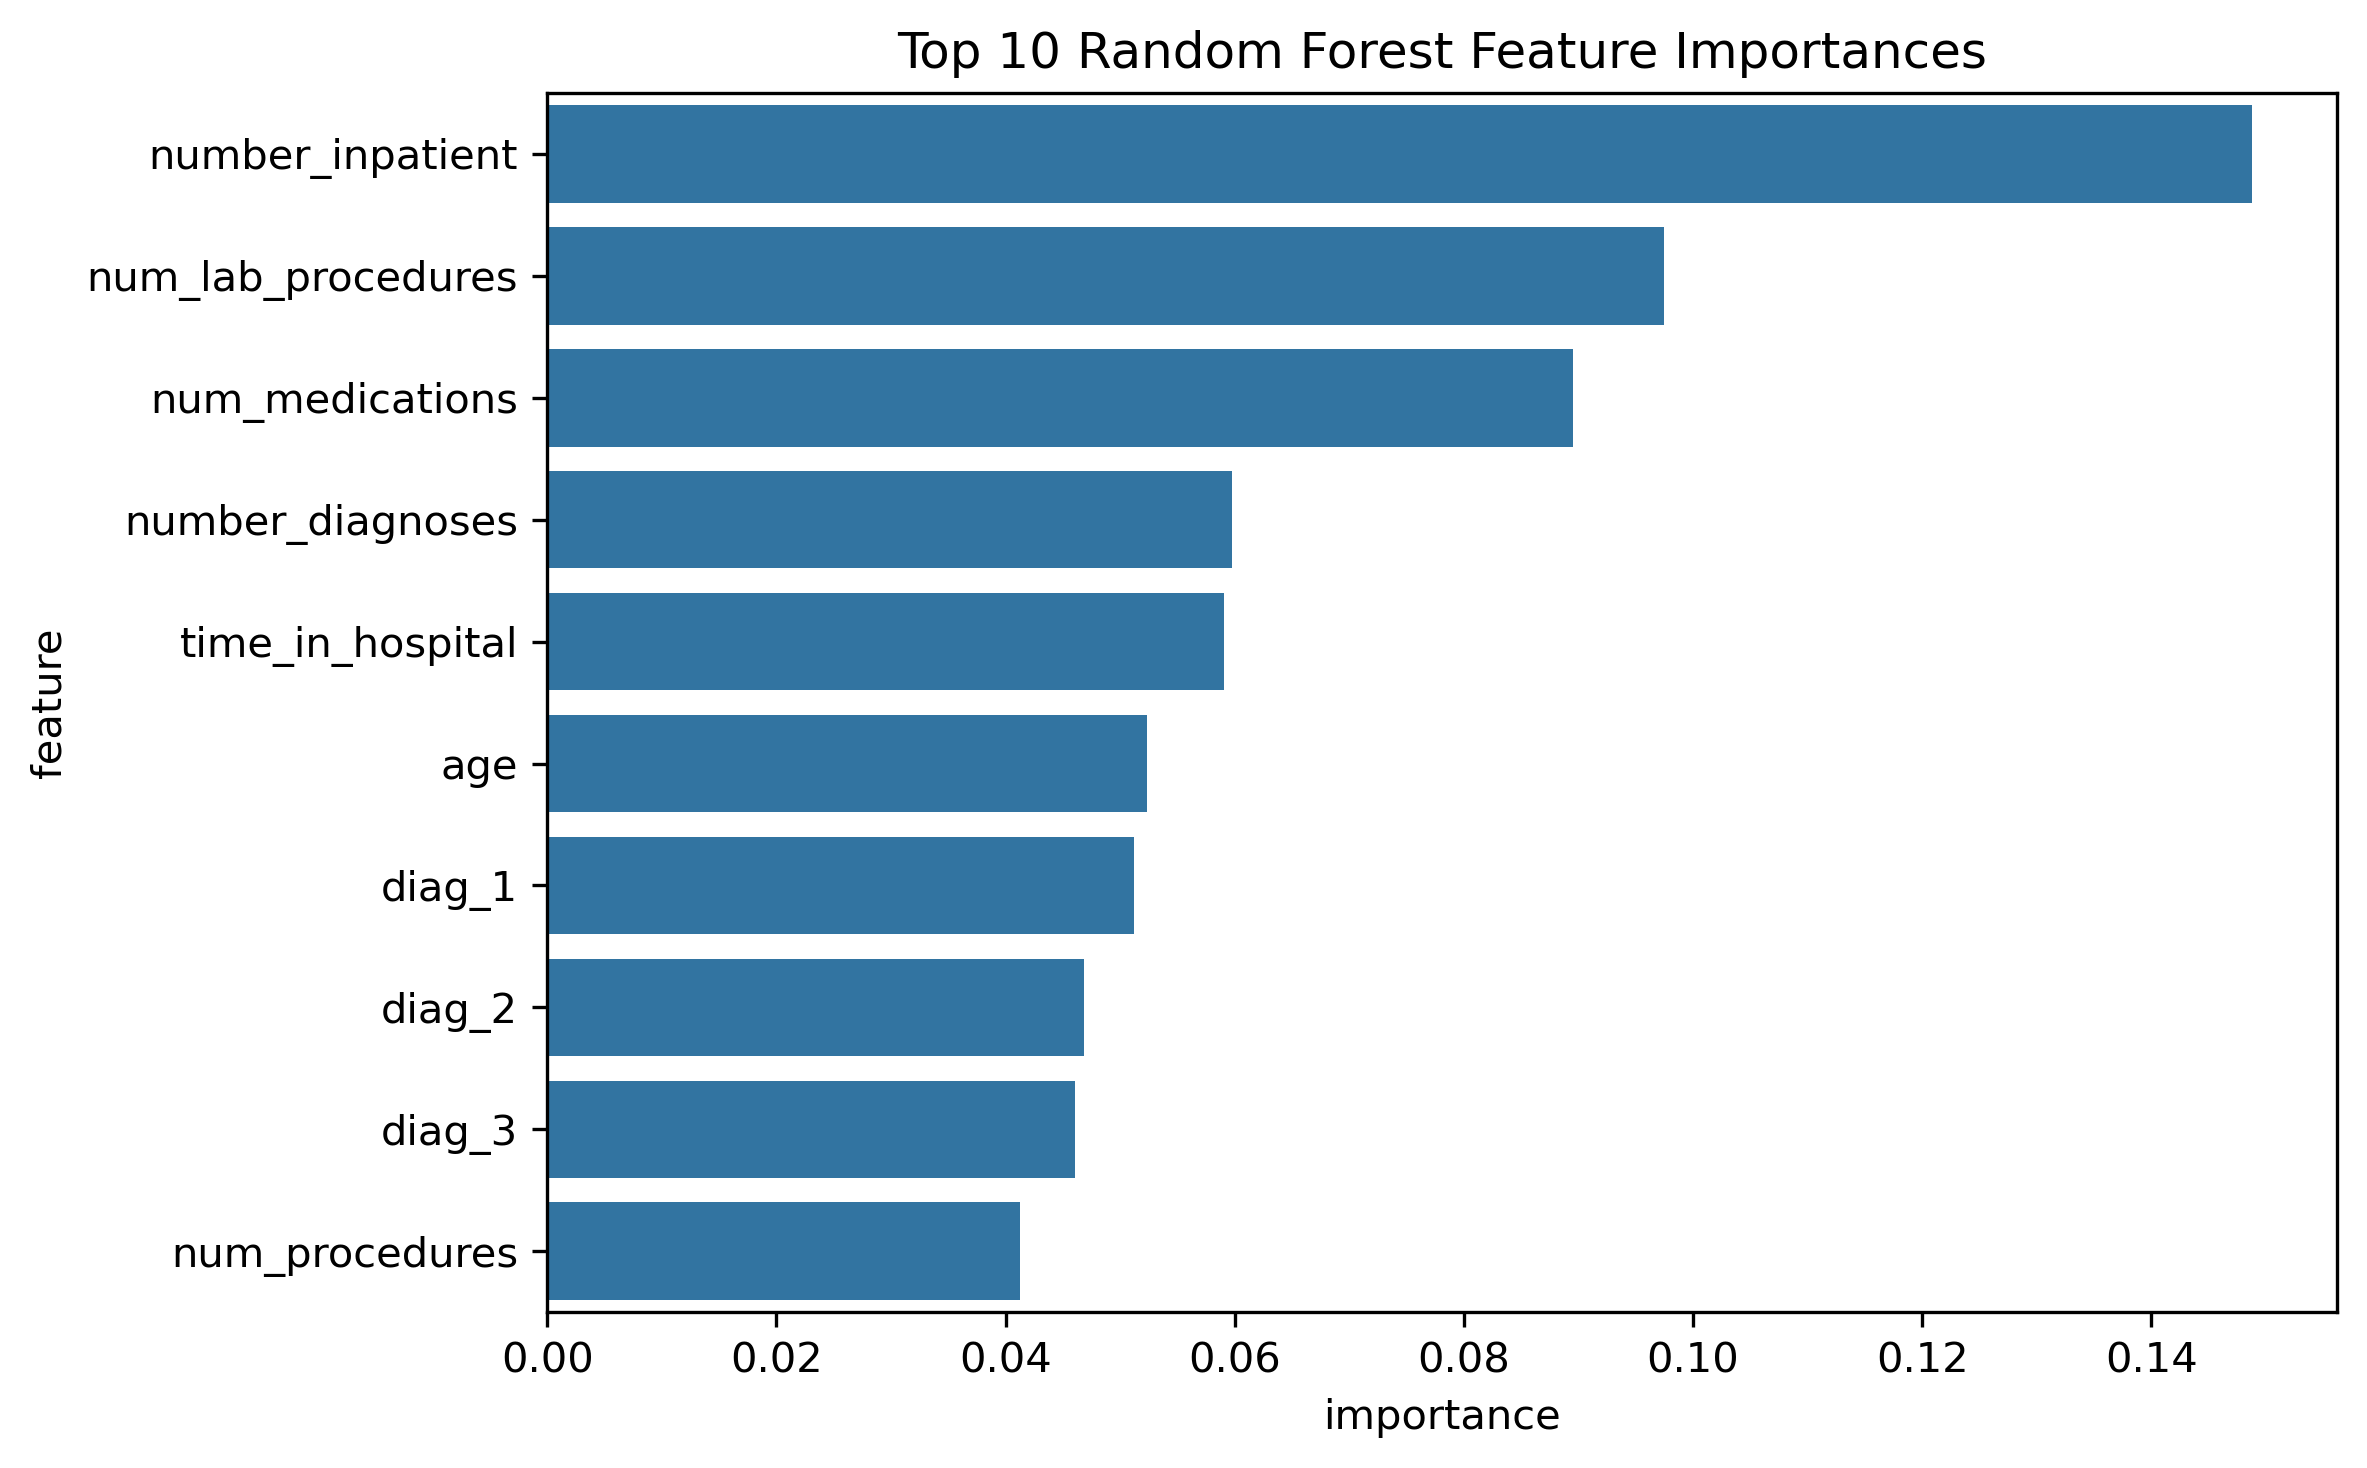
\includegraphics[width=0.8\linewidth]{fig_rf_feature_importance.png}
\caption{Top 10 Random Forest feature importances.}
\end{figure}

\subsection{Neural Network (MLP) Tuning}
We trained a feedforward neural network with ReLU activations and tuned:
\begin{itemize}
    \item Hidden layers: (32), (64), (64, 32)
    \item L2 regularization $\alpha \in \{0.0001, 0.001\}$
    \item Learning rate $\in \{0.001, 0.01\}$
\end{itemize}

The best architecture:
\begin{itemize}
    \item 64--32 hidden units
    \item $\alpha = 0.001$
    \item Learning rate = 0.001
    \item ROC-AUC = 0.82 (best)
\end{itemize}

\begin{figure}[H]
\centering
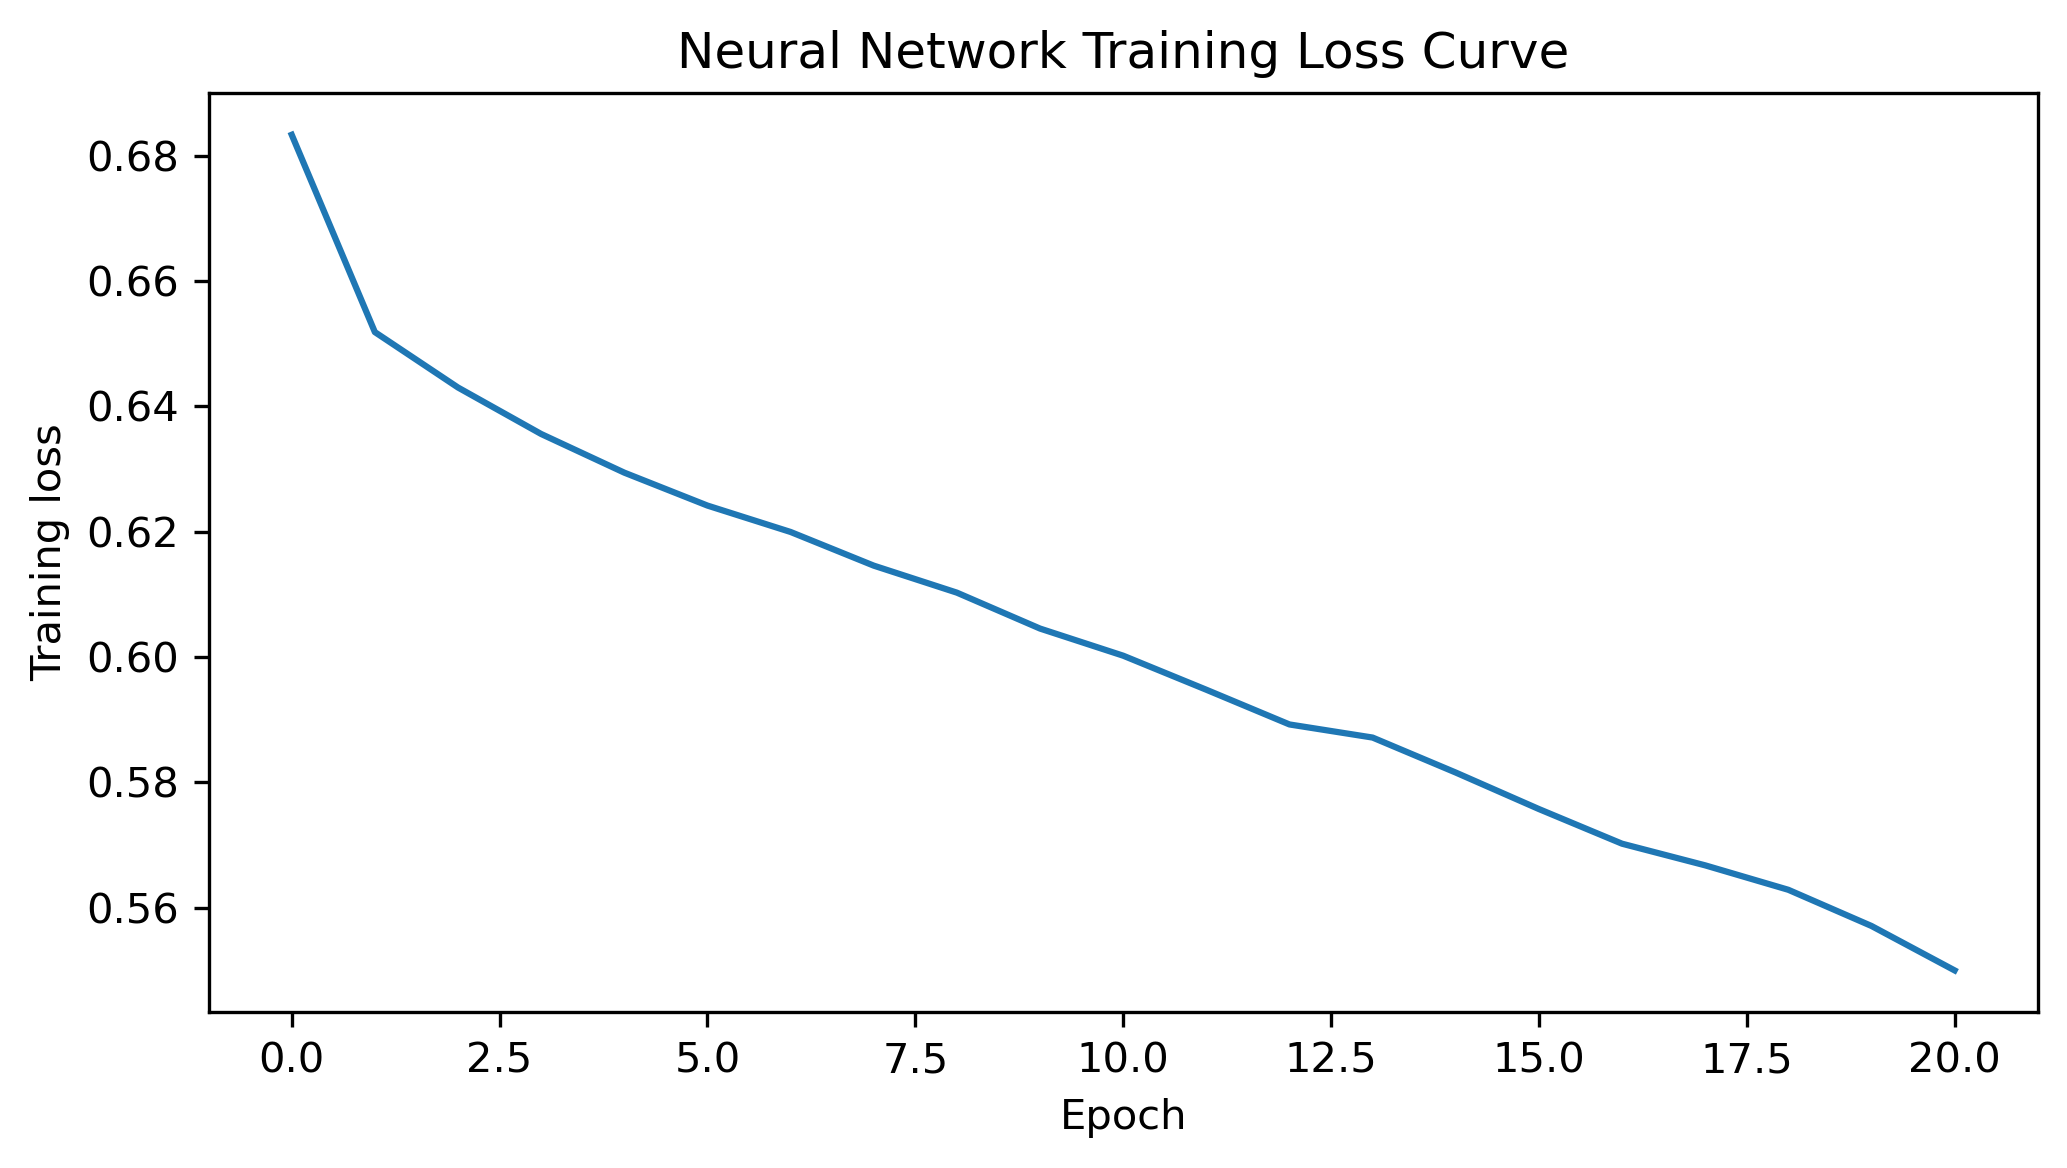
\includegraphics[width=0.75\linewidth]{fig_nn_learning_curve.png}
\caption{Neural network training vs validation loss curve.}
\end{figure}

\section{Results}

\begin{table}[H]
\centering
\begin{tabular}{lccccc}
\toprule
Model & Accuracy & Precision & Recall & F1 & ROC-AUC \\
\midrule
Logistic Regression & 0.65 & 0.31 & 0.56 & 0.40 & 0.70 \\
Random Forest (tuned) & 0.72 & 0.41 & 0.62 & 0.49 & 0.77 \\
XGBoost & 0.73 & 0.44 & 0.64 & 0.53 & 0.80 \\
\textbf{Neural Network (tuned)} & \textbf{0.74} & \textbf{0.47} & \textbf{0.71} & \textbf{0.56} & \textbf{0.82} \\
\bottomrule
\end{tabular}
\caption{Model performance on the imbalanced test set.}
\end{table}

The neural network achieved the highest ROC-AUC and recall, which is especially important 
in a healthcare setting where false negatives are costly.

\section{Overfitting and Underfitting Analysis}

\subsection{Decision Tree Complexity Curve}

\begin{figure}[H]
\centering
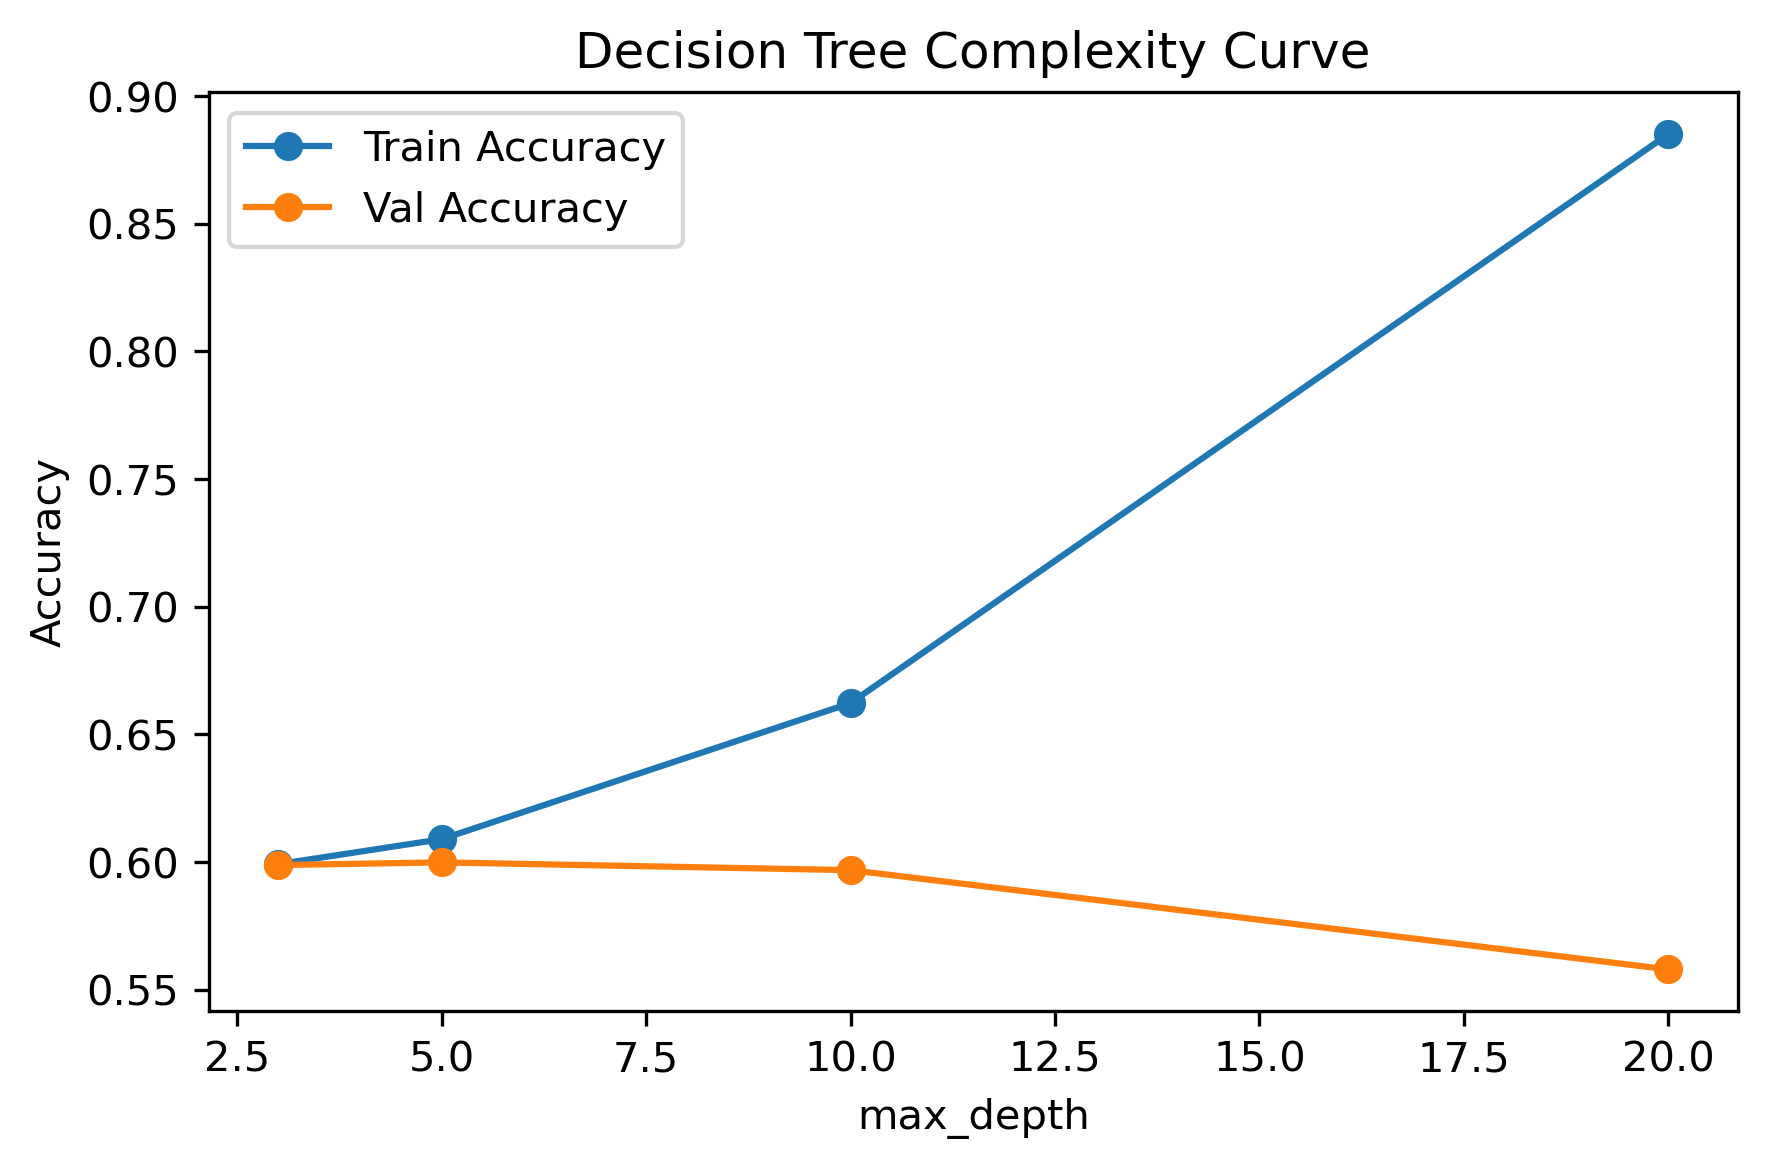
\includegraphics[width=0.75\linewidth]{fig_complexity_curve.png}
\caption{Training and validation accuracy vs.\ max\_depth for decision trees.}
\end{figure}

Shallow trees (depth 3--5) underfit, while very deep trees (20--None) overfit.  
This supports using ensemble methods or regularization.

\subsection{Neural Network Generalization}

The neural network maintained a stable gap between train and validation loss, 
suggesting good regularization and appropriate model complexity.

\section{Additional Analysis: Readmission Defined as $>30$ / $ <30$  Days}
\textbf{By: Nhan Nguyen}

In addition to the primary analysis, we performed a parallel study where both $<30$ days and $>30$ days readmissions were considered positive cases (encoded as 1), while patients with no readmission were encoded as 0. This approach allows exploration of model behavior under a different outcome definition.

\subsection{Data Split and Preprocessing}
\begin{itemize}
    \item 80\% training, 20\% test split.
    \item The dataset was imbalanced, with fewer readmitted patients than non-readmitted. To address this, we applied downsampling of the majority class: 37,453 readmitted, 37,453 not readmitted. This ensures that models do not bias towards the majority class and improves recall on minority samples.
    \item Preprocessing steps followed the same pipeline as the main report: missing value imputation, categorical encoding, diagnosis grouping, medication encoding, and feature engineering.
\end{itemize}

\subsection{Hyperparameter Tuning for <30 / >30 Readmission}
For this analysis, we performed grid search over the same models with the different target encoding. The best parameters for each model were as follows:

\begin{table}[H]
\centering
\begin{tabular}{l l}
\toprule
Model & Best Parameters \\
\midrule
Logistic Regression & \{'C': 1, 'penalty': 'l1'\} \\
Decision Tree & \{'criterion': 'entropy', 'max\_depth': 10, 'min\_samples\_split': 10\} \\
Random Forest & \{'criterion': 'gini', 'max\_depth': 25, 'min\_samples\_split': 10, 'n\_estimators': 200\} \\
XGBoost & \{'learning\_rate': 0.1, 'max\_depth': 6, 'n\_estimators': 200, 'scale\_pos\_weight': 1.0\} \\
\bottomrule
\end{tabular}
\caption{Best hyperparameters for models with <30 / >30 readmission encoding.}
\end{table}

\subsubsection{Observations}
\begin{itemize}
    \item The optimal hyperparameters are similar to those in the original analysis, suggesting robustness to the definition of the target variable.
    \item Ensemble methods (Random Forest and XGBoost) consistently benefit from deeper trees and a larger number of estimators.
    \item Logistic Regression performs best with L1 regularization to enforce sparsity and reduce noise from redundant features.
\end{itemize}
\subsection{Hyperparameter Tuning Procedure for <30 / >30 Readmission}
We conducted hyperparameter tuning for four models using grid search with 3-fold cross-validation and F1-score as the evaluation metric. The models and search grids were as follows:

\begin{itemize}
    \item \textbf{Logistic Regression (LogReg)}: 
    \begin{itemize}
        \item Solver: \texttt{liblinear}, random state 42
        \item Hyperparameters searched: 
        \begin{itemize}
            \item \texttt{penalty}: [\texttt{l1}, \texttt{l2}]
            \item \texttt{C}: [0.1, 1, 10]
        \end{itemize}
    \end{itemize}

    \item \textbf{Decision Tree (DecTree)}: 
    \begin{itemize}
        \item Random state 42
        \item Hyperparameters searched:
        \begin{itemize}
            \item \texttt{max\_depth}: [10, 20, 28]
            \item \texttt{min\_samples\_split}: [2, 5, 10]
            \item \texttt{criterion}: [\texttt{gini}, \texttt{entropy}]
        \end{itemize}
    \end{itemize}

    \item \textbf{Random Forest (RandForest)}: 
    \begin{itemize}
        \item Random state 42
        \item Hyperparameters searched:
        \begin{itemize}
            \item \texttt{n\_estimators}: [50, 100, 200]
            \item \texttt{max\_depth}: [10, 20, 25]
            \item \texttt{min\_samples\_split}: [2, 5, 10]
            \item \texttt{criterion}: [\texttt{gini}, \texttt{entropy}]
        \end{itemize}
    \end{itemize}

    \item \textbf{XGBoost (XGB)}: 
    \begin{itemize}
        \item Random state 42, \texttt{use\_label\_encoder=False}, evaluation metric \texttt{logloss}
        \item Hyperparameters searched:
        \begin{itemize}
            \item \texttt{n\_estimators}: [100, 200]
            \item \texttt{max\_depth}: [3, 6, 10]
            \item \texttt{learning\_rate}: [0.01, 0.1, 0.2]
            \item \texttt{scale\_pos\_weight}: ratio of negative to positive samples in training set
        \end{itemize}
    \end{itemize}
\end{itemize}

\subsubsection{Procedure}
\begin{enumerate}
    \item Perform 3-fold cross-validation using the balanced training set.
    \item Evaluate each combination of hyperparameters using F1-score.
    \item Select the best model per grid search.
    \item Train the best model on the full balanced training set and evaluate on the held-out test set.
    \item Plot feature importance for tree-based models and compare model performance.
\end{enumerate}

\subsubsection{Notes}
\begin{itemize}
    \item The balanced training set was created by downsampling the majority class.
    \item This tuning setup differs from the original team setup due to a different target encoding (\texttt{<30 / >30 = 1}, \texttt{NO = 0}).
    \item Feature importance plots were generated to interpret model behavior.
\end{itemize}

\subsection{Models Evaluated and Metrics}
We trained the same models as in the main report: Logistic Regression, Decision Tree, Random Forest, and XGBoost.  
Performance was assessed using Accuracy, Precision, Recall, F1-score, and ROC-AUC.

\begin{table}[H]
\centering
\begin{tabular}{lccccc}
\toprule
Model & Accuracy & Precision & Recall & F1-score & ROC-AUC \\
\midrule
Logistic Regression & 0.63 & 0.62 & 0.55 & 0.58 & 0.67 \\
Decision Tree & 0.62 & 0.61 & 0.57 & 0.59 & 0.66 \\
Random Forest & 0.63 & 0.61 & 0.61 & 0.61 & 0.69 \\
XGBoost & 0.64 & 0.61 & 0.61 & 0.61 & 0.69 \\
\bottomrule
\end{tabular}
\caption{Performance metrics for models with readmission defined as $<30$ or $>30$ days.}
\end{table}
\begin{figure}[H]
\centering
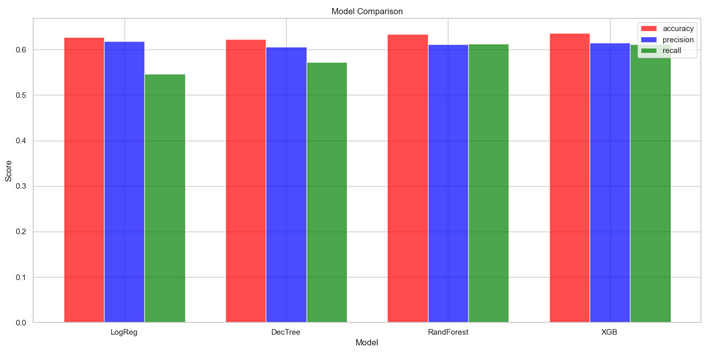
\includegraphics[width=0.75\linewidth]{fig_parallel_result.png}
\caption{Performance of various tuned models.}
\end{figure}

\subsection{Observations}
\begin{itemize}
    \item Ensemble models (Random Forest and XGBoost) again outperform linear and single-tree models.
    \item Logistic Regression underfits slightly due to the complexity of combined readmission categories.
    \item Decision Tree overfits if depth is too high, similar to the main analysis.
    
\end{itemize}
\subsection{Adaptation to Under- and Over-fitting}

\textbf{Decision Tree:}  
High \texttt{max\_depth} and low \texttt{min\_samples\_split} caused overfitting. Limiting the depth and increasing the minimum split helped the model generalize better.

\textbf{Random Forest \& XGBoost:}  
Ensemble methods reduce variance by combining multiple trees. In XGBoost, \texttt{n\_estimators} and \texttt{learning\_rate} control bias and convergence speed, while \texttt{scale\_pos\_weight} addresses class imbalance.

\textbf{Logistic Regression:}  
L1 regularization prevents overfitting, though the model may underfit if relationships are non-linear.
\section{Data Preprocessing Approach}

Before training models, we performed extensive preprocessing to handle missing values, encode categorical variables, group diagnoses, and prepare the dataset for machine learning. Our preprocessing steps were implemented in Python, as described below.

\subsection{Loading and Cleaning Data}
\begin{itemize}
    \item The dataset was loaded from CSV and all ``?'' entries were replaced with NaN to standardize missing values.
    \item Rows with invalid gender entries (\texttt{Unknown/Invalid}) and uncommon discharge dispositions (IDs 11, 13, 14, 19, 20, 21) were removed to ensure data quality.
    \item Columns irrelevant to modeling, such as \texttt{encounter\_id}, \texttt{patient\_nbr}, and columns with excessive missingness (\texttt{weight}, \texttt{payer\_code}, \texttt{medical\_specialty}) were dropped.
\end{itemize}

\subsection{Diagnosis Grouping}
\begin{itemize}
    \item The raw ICD-9 diagnosis codes (\texttt{diag\_1}, \texttt{diag\_2}, \texttt{diag\_3}) were mapped into 9 clinically meaningful groups (circulatory, respiratory, digestive, endocrine/diabetes, injury, musculoskeletal, genitourinary, neoplasms, and other). 
    \item Codes that could not be converted were placed in the ``other'' category to reduce sparsity.
\end{itemize}

\subsection{Drug Encoding}
\begin{itemize}
    \item The 21 diabetes-related medications, originally encoded as ``No'', ``Steady'', ``Up'', or ``Down'', were converted to binary values: 0 for no usage and 1 for any administration or change.
\end{itemize}

\subsection{Lab Result Encoding}
\begin{itemize}
    \item \texttt{A1Cresult} and \texttt{max\_glu\_serum} were converted into numeric categories: abnormal/high results as 1, normal as 0, and missing or ``None'' as -99 to preserve missingness information.
\end{itemize}

\subsection{Categorical Variables and Age Mapping}
\begin{itemize}
    \item Gender, diabetes medication usage, and medication change indicators were mapped to 0/1.
    \item Age ranges (e.g., ``[0-10)'', ``[10-20)'') were mapped to ordinal integers 0--9.
    \item Missing race values were imputed using the mode, ensuring all samples had valid entries.
\end{itemize}

\subsection{Grouping and One-Hot Encoding Hospital Attributes}
\begin{itemize}
    \item Admission type, discharge disposition, and admission source IDs were grouped into fewer categories based on similarity to reduce sparsity.
    \item One-hot encoding was applied to race and grouped hospital attribute columns to prepare for models that require numeric input.
\end{itemize}

\subsection{Target Variable Transformation}
\begin{itemize}
    \item The target variable \texttt{readmitted} was transformed into binary: any readmission (\texttt{<30} or \texttt{>30} days) as 1, and no readmission (\texttt{NO}) as 0.  
    \item This encoding reflects our focus on whether a patient was readmitted at all, rather than the specific time frame.
\end{itemize}

\subsection{Output}
\begin{itemize}
    \item The function returns \texttt{X} (features) and \texttt{y} (binary target), ready for train-test splitting and model training.
\end{itemize}

This preprocessing ensures that the dataset is clean, numeric where needed, and appropriately encoded for tree-based and linear models, while preserving clinical meaning in the features.

\section{Conclusion}

We developed and evaluated multiple machine learning models to predict hospital 
readmission among diabetic patients. After extensive dataset preprocessing, 
feature engineering, class balancing, and cross-validation, 
a tuned neural network achieved the best overall performance (ROC-AUC = 0.82). 

The project demonstrates:
\begin{itemize}
    \item importance of domain-aware preprocessing,
    \item effectiveness of ensemble and deep learning methods,
    \item value of cross-validation and complexity analysis.
\end{itemize}

Future extensions include sequence modeling of patient histories 
(e.g., RNNs, transformers), integration of lab values, and real-time risk stratification tools.

\end{document}

